\section*{Задание:}
Научиться работать с LaTex и GitHub.
%\addcontentsline{toc}{section}{Введение} добавляет строчку в оглавление
\begin{enumerate}

    \item{Завести профиль на GitHub. Рис. 1}

\begin{figure}[h]%подключаем фото (его нужно класть в шаблон>src>img>*.png и главное png обязательно) в [] пишем ключ рендра т.е b отображаеться в конце файла h там где вставляем
\centering
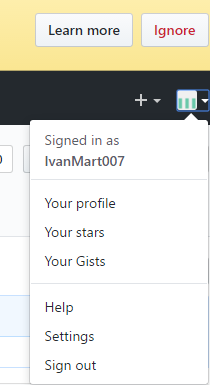
\includegraphics[scale=1]{ccountgit}%scale это размер отображаемого фото,а в {} имя файла
\caption{Профиль на Git.}
\label{fig:ccountgit}
\end{figure}

\item{Склонировать репозиторий шаблонов tex.Рис. 2}


%\renewcommand{\theenumi}{\arabic{enumi})}

\begin{figure}[h]
    \centering
    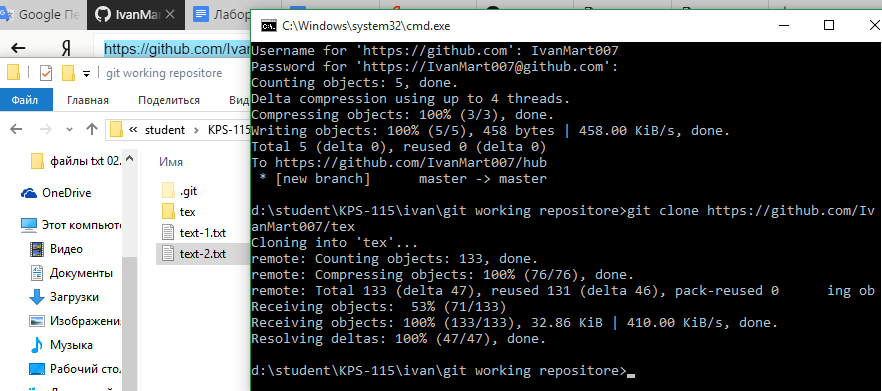
\includegraphics[scale=0.5]{git_clone}
    \caption{Копирование репозитория Git.}
    \label{fig:git_clone}
\end{figure}


\item{Создать новый репозиторий для лабораторных работ на гитхабе.Рис.3}
\end{enumerate}

\newpage


\renewcommand{\theenumi}{\arabic{enumi})}
\begin{figure}[h]
\centering
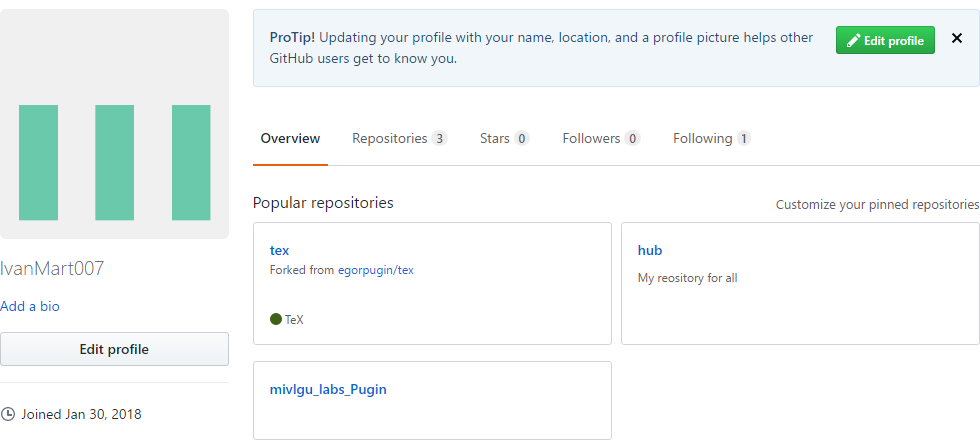
\includegraphics[scale=0.5]{screengit}
\caption{Список репозиториев на Git.}
\label{fig:screengit}
\end{figure}




\long\def\comment{% позволяет делать коментарии
}

\textbf{Вывод:} Я научился работать с git и LaTex приобрёл навыки работы с TeXstudio.
